% LaTeX source for ``การเรียนรู้ของเครื่องสำหรับเคมีควอนตัม (Machine Learning for Quantum Chemistry)''
% Copyright (c) 2022 รังสิมันต์ เกษแก้ว (Rangsiman Ketkaew).

% License: Creative Commons Attribution-NonCommercial-NoDerivatives 4.0 International (CC BY-NC-ND 4.0)
% https://creativecommons.org/licenses/by-nc-nd/4.0/

\chapter{โมเดลการเรียนรู้ของเครื่องสำหรับเคมีควอนตัม}
\label{ch:chem_ml}

%--------------------------
\section{ANI-1}
\idxen{Model for Quantum Chemistry!ANI-1}
%--------------------------

ANI เป็นชื่อย่อสั้น ๆ ของโมเดล ANAKIN-ME ซึ่งย่อมาจาก Accurate NeurAl networK engINe for Molecular Energies อีกทีหนึ่ง 
โดยโมเดลตัวนี้ถูกพัฒนาด้วย Neural Network สำหรับการทำนายค่าพลังงานศักย์ของโมเลกุลโดยที่มีความแม่นยำในระดับเดียวกับการคำนวณด้วยวิธี 
DFT\autocite{smith2017a}

%--------------------------
\section{SchNet และ SchNOrb}
%--------------------------

%--------------------------
\subsection{SchNet}
\idxen{Model for Quantum Chemistry!SchNet}
%--------------------------

\autocite{schutt2017,schutt2018}

%--------------------------
\subsection{SchNOrb}
\idxen{Model for Quantum Chemistry!SchNOrb}
%--------------------------

SchNOrb ย่อมาจาก \enquote{SchNet for Orbitals}\autocite{schutt2019a}

%--------------------------
\section{GDML และ sGDML}
%--------------------------

%--------------------------
\subsection{GDML}
\idxen{Model for Quantum Chemistry!GDML}
%--------------------------

\autocite{chmiela2017}

%--------------------------
\subsection{sGDML}
\idxen{Model for Quantum Chemistry!sGDML}
%--------------------------

\autocite{chmiela2018}

\autocite{sauceda2020}

%--------------------------
\section{$\Delta$ML}
\idxen{Model for Quantum Chemistry!$\Delta$ML}
%--------------------------

งานวิจัยที่ใช้ Correction หรือผลต่างของผลลัพธ์จากการคำนวณและค่าอ้างอิงมาช่วยทำให้การทำนายคุณสมบัติของโมเลกุลมีค่าแม่นยำมากยิ่งขึ้นนั้น%
นั้นมีมานานแล้ว\autocite{hu2003,wu2007,balabin2009}

Delta-ML ($\Delta$ML) เป็นเทคนิคที่ใช้ค่าความแตกต่างระหว่างค่าอ้างอิง (Reference หรือจะเรียก Label ก็ได้) จากวิธีการคำนวณที่มีความ%
แม่นยำต่ำกับความแม่นยำสูงมาใช้ในการเทรนโมเดล (จึงเป็นที่มาว่าทำไมถึงเรียกว่า Detla) ซึ่งการทำแบบนี้จะช่วยให้โมเดลสามารถเรียนรู้การเชื่อมโยง 
(Transferability) ไปยังค่าที่ต้องการทำนายได้อย่างถูกต้องและแม่นยำมากขึ้น โดยจะมีความถูกต้องเทียบเคียงกับการใช้วิธีแบบดั้งเดิมที่มีความแม่นยำสูง 
(เช่น Post-HF) ตัวอย่างของการใช้ $\Delta$ML คือการใช้ค่าความแตกต่างของพลังงานที่ได้จากการคำนวณด้วยวิธี DFT และ CCSD(T) 
($y_{\text{DFT}} - y_{\text{CCSD(T)}}$) มาฝึกสอนโมเดล\autocite{ramakrishnan2015a} นอกจอกนี้ยังมีงานวิจัยที่พัฒนา Graph 
Neural Network (GNN) และประยุกต์ใช้เข้ากับเทคนิค $\Delta$-learning สำหรับการประมาณค่าพลังงานส่วนต่างของเทอม Triple excitation
(correction) เพื่อเพิ่มความแม่นยำในการทำนายค่าพลังงานให้มีความแม่นยำในระดับเดียวกันหรือใกล้เคียงกับวิธี CCSD(T)\autocite{ruth2022}

จริง ๆ แล้ว $\Delta$ML ก็เป็นเทคนิคอันนึงที่มีแนวคิดมาจากความพยายามที่ต้องการจะทำให้โมเดลสามารถเรียนรู้ได้จากค่าความผิดพลาด (Error) 
โดยเริ่มมีการเอามาใช้กันมากขึ้นในช่วงปีที่ผ่านมา (ในช่วงแรกถูกใช้เยอะแค่ในเฉพาะกลุ่มวิจัยในโซนยุโรป สำหรับการเอามาทำนายพลังงานและ%
เกรเดียนต์ของพลังงาน (Energy Gradient) ซึ่งก็สอดคล้องกับแรงของแต่ละอะตอมในโมเลกุลโมเลกุลนั่นเอง

%--------------------------
\section{Graph Neural Network}
\idxth{โครงข่ายประสาทแบบกราฟ}
\idxen{Graph Neural Network}
%--------------------------

โครงข่ายประสาทแบบกราฟ (Graph Neural Network หรือ GNN) เป็นโครงข่ายประสามแบบหนึ่งซึ่งจะมองความสัมพันธ์ภายในโครงสร้างข้อมูลให้%
อยู่ในรูปแบบของกราฟแบบ 2 มิติ โดยไอเดียนี้ได้ถูกเสนอตั้งแต่ปี ค.ศ. 2008\autocite{scarselli2009,zhou2020}

\begin{figure}[H]
    \centering
    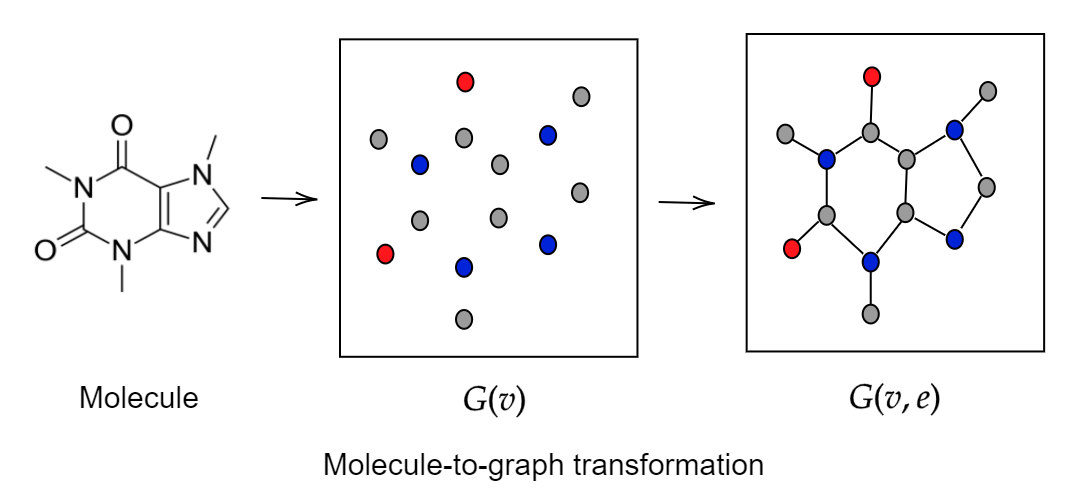
\includegraphics[width=\linewidth]{fig/mol-2-graph.png}
    \caption{การแทนโมเลกุลด้วยกราฟ}
    \label{fig:mol_2_graph}
\end{figure}

ภาพ \ref{fig:mol_2_graph} แสดงกราฟฟิคของการเปรียบเทียบโมเลกุลและกราฟ ซึ่งจะเห็นได้ว่าการแปลงจากโมเลกุลไปเป็นกราฟนั้นสามารถ%
ทำได้ตรงไปตรงมาเพราะว่าเราสามารถแทนอะตอมด้วยโหนด (Node) หรือจุดยอดของกราฟ (Vertex) และแทนพันธะด้วยขอบ (Edge)

%--------------------------
\subsection{Message Passing Neural Network}
\idxth{โครงข่ายประสาทแบบการส่งข้อความ}
\idxen{Message Passing Neural Network}
%--------------------------

โครงข่ายประสาทแบบการส่งข้อความ (Message Passing Neural Network หรือ MPNN) เป็น GNN ประเภทหนึ่งซึ่งถูกนำเสนอครั้งแรกเมื่อปี 
ค.ศ. 2017\autocite{gilmer2017} โดยที่ MPNN แบบฉบับดั้งเดิมนั้นจะเป็นการใช้กราฟแบบที่ไม่มีการนำทิศทางหรือ Undirected Graph
ซึ่ง MPNN นั้นประกอบไปด้วยเฟสหลัก 2 เฟส ดังนี้ 

\begin{itemize}
    \item Message passing phase เฟสการส่งผ่านข้อความ (ข้อมูล) เป็นเฟสที่จะทำการขยับหรือแผ่กระจายข้อมูลไปทั่วทั้งกราฟเพื่อจำลองการ%
    เกิดโครงข่ายประสาทและการส่งต่อข้อมูลจากโหนดหนึ่งไปยังอีกโหนดหนึ่ง
    \item Readout phase เฟสการเรียกใช้ข้อมูล เป็นเฟสที่ Neural Representation ของกราฟจะถูกใช้ในการทำนายค่าของเอาต์พุต เช่น
    คุณสมบัติของแต่ละโหนด ซึ่งเปรียบเสมือนการทำนายคุณสมบัติของแต่อะตอมแต่ละตัวในโมเลกุลนั่นเอง
\end{itemize}

\begin{figure}[H]
    \centering
    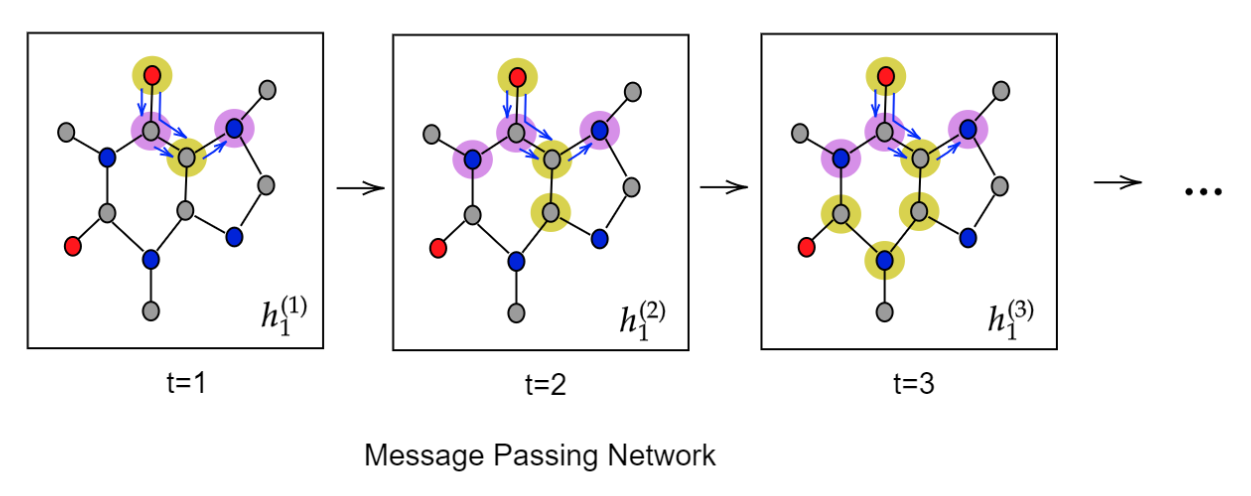
\includegraphics[width=\linewidth]{fig/mp-network.png}
    \caption{โครงข่ายของการส่งข้อความ}
    \label{fig:mp_network}
\end{figure}

เรามาดูรายละเอียดของเฟสแรกกันครับ เฟสแรกนั้นจะเป็นการดำเนินการแผ่กระจายข้อมูลทั่วทั้งกราฟ โดยจำนวนก้าวที่ใช้ในการทำ Propagation 
นั้นจะเขียนแทนด้วย $T$ ซึ่งจริง ๆ แล้วก็คือจำนวนรอบของการฝึกสอนโมเดล (Iteration) นั่นเอง นอกจากนี้เรายังกำหนดตัวแปรแทนพารามิเตอร์%
อื่น ๆ อีก ดังนี้

\begin{description}[font=$\bullet$]
    \item[$h$] สถานะซ่อน
    \item[$m^{t}_{v}$] ข้อความของโหนด $v$ ณ สเต็ปที่ $t$
    \item[$M$] ฟังก์ชันที่ใช้ในการอัพเดทข้อความ
    \item[$U_{t}$] ฟังก์ชันที่ใช้ในการอัพเดทโหนด ณ สเต็ปที่ $t$    
\end{description}

ซึ่งฟังก์ชันที่ใช้ในการอัพเดทข้อความของแต่ละเสต็ปที่เกิดขึ้นในการกระบวน Propagation นั้นมีหน้าตาดังนี้

\begin{equation}\label{eq:msg_func}
    m^{t+1}_{v} = \sum_{w \in N(v)} M_{t} (h^{t}_{v}, h^{t}+{w}, e_{vw})
\end{equation}

\noindent ถ้าเราสังเกตสมการข้างต้นดี ๆ จะพบว่าฟังก์ชัน $m$ จะมีการดำเนินการนำข้อมูลของสถานะซ่อน (Hidden States) ของโหนด $w$ 
เข้าไปกระทำกับโหนด $v$ และยังมีการนำข้อมูลของขอบระหว่างโหนด $e_{vw}$ เข้ามารวมไว้ในฟังก์ชันด้วย นอกจากนี้สมการทางคณิตศาสตร์ของ 
Hidden State สามารถเขียนให้อยู่ในรูปของฟังก์ชันที่ใช้อัพเดทสถานะของแต่ละโหนดได้ดังนี้ 

\begin{equation}\label{hidden_func}
    h^{t+1}_{v} = U_{t}(h^{t}_{v}, m^{t+1}_{v})
\end{equation}

\noindent โดยที่ $N(v)$ คือเซตของโหนดข้างเคียงของโหนด $v$ ในกราฟ $G$ และ $h^{0}_{v}$ คือฟังก์ชันเริ่มต้น (ฟังก์ชันอะไรก็ได้) 
สำหรับการกำหนดค่าเริ่มต้นของข้อมูลของโหนดนั้น ๆ (กำหนด Feature) $x_{v}$

\begin{center}
\fbox{\begin{minipage}{0.8\linewidth}
    $\phi_{1 \rightarrow 3} = f(v_{1} \rightarrow v_{3})$ \\
    $\psi_{2 \rightarrow 3} = f(v_{2} \rightarrow v_{3})$ \\
    \hspace{2em} Summarize messages: $\Omega = \phi_{1 \rightarrow 3} \,\, \& \,\, \psi_{2 \rightarrow 3}$ \\
    \\
    $h^{t+1}_{v} = \text{Update}(h^{t}_{v}, \Omega )$
\end{minipage}}
\end{center}

เมื่อเรามีสถานะซ่อนของแต่ละโหนด ณ เวลาที่แตกต่างกันแล้ว ($h^{t}_{v}$) ลำดับถัดมาคือเราต้องการดำเนินการถดถอย (Regress) สถานะซ่อน%
ทั้งหมดนี้เพื่อคำนวนความสัมพันธ์ไปยังค่าเอาต์พุตนั่นเอง ซึ่งกระบวนการหรือสิ่งที่เราจะนำมาใช้ในการทำดังกล่าวคือต้องใช้ฟังก์ชัน Readout $R$ นั่นเอง
หรือพูดง่าย ๆ คือเป็นฟังก์ชันที่ใช้ในการถอดข้อความออกมาเป็นเอาต์พุต เรียกว่าการทำนายสถานะซ่อน โดยมีสมการดังต่อไปนี้

\begin{equation}
    \hat{y} = R({h^{T}_{v} | v \in G})
\end{equation}

\noindent ฟังก์ชัน Readout ที่เราจะนำมาใช้นั้นจะเป็นฟังก์ชันอะไรก็ได้ ขอแค่สามารถรวบรวม (Compose) ข้อความทั้งหมดที่อยู่ในรูปของสถานะซ่อน%
เข้าไว้ด้วยกันและทำการผสาน (Merge) ข้อความเหล่านั้นให้เป็น $\hat{y}$ ซึ่งฟังก์ชันแบบที่ง่ายที่สุดก็คือการรวมสถานะต่าง ๆ เข้าไว้ด้วยกันแบบเชิงเส้น

\begin{equation}
    h = \sum_{v \in G} h^{T}_{v}
\end{equation}

\begin{equation}\label{eq:ff_mpnn}
    \hat{y} = f(h)
\end{equation}

สุดท้ายแล้วการฝึกสอนโมเดล MPNN สิ่งที่เราก็คือฟังก์ชันที่รับสถานะของแต่ละโหนดเข้ามาที่ผ่านการแผ่กระจายมาจากโหนดอื่น ๆ โดยผ่านขอบระหว่างโหนด 
แล้วทำการรวมข้อมูลและแปลงให้เป็นคำตอบที่ต้องการทำนาย สมการที่ \ref{eq:ff_mpnn} ก็คือการฝึกสอนโมเดล Feed-Forward Neural Network 
โดยใช้ฟังก์ชันไม่เชิงเส้น (Non-linear) $f$

\begin{figure}[H]
    \centering
    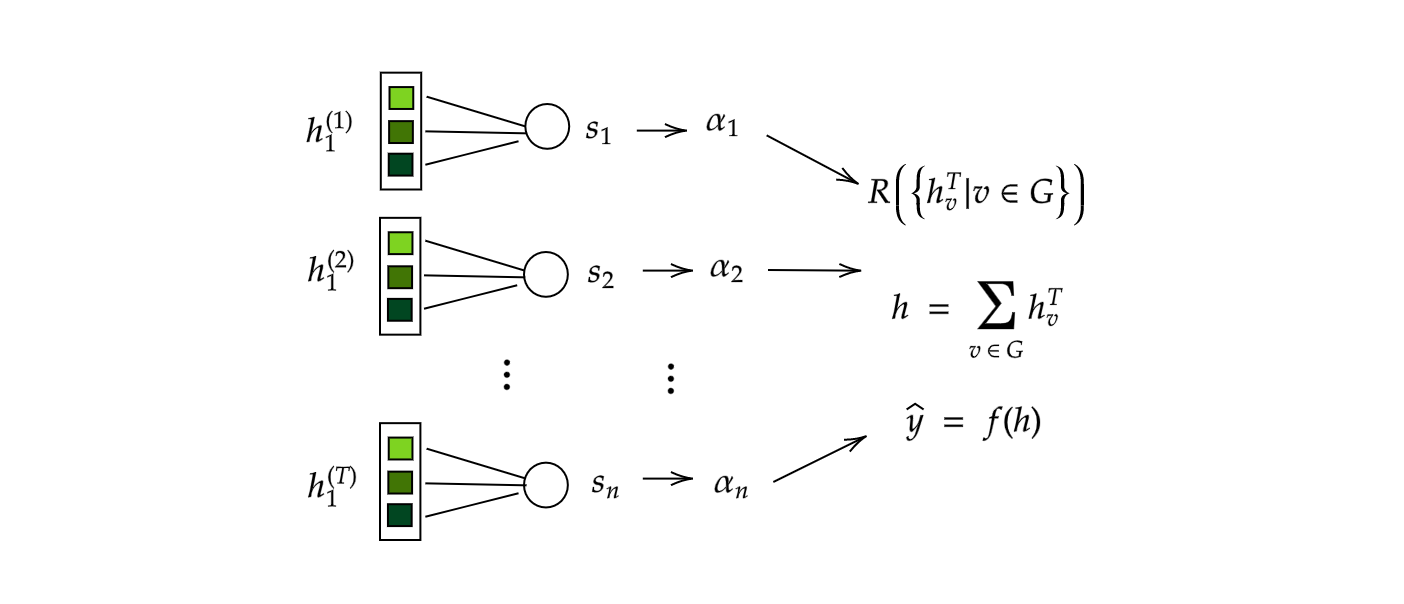
\includegraphics[width=1.2\linewidth]{fig/mp-operation.png}
    \caption{การดำเนินการของการทำการถดถอย (Regression) และการเรียกหรือดึงข้อมูลโดยใช้ Readout}
    \label{fig:mp_operation}
\end{figure}

สำหรับ Representation ของโมเลกุลที่เราสามารถเลือกใช้เพื่อนำฝึกสอนโมเดล MPNN นั้นจะแบ่งออกได้ง่าย ๆ ตามลักษณะองค์ประกอบของกราฟ 
นั่นคือ \textit{โหนด} ซึ่งเรามองเห็นอะตอม และ \textit{ขอบ} ซึ่งเรามองเห็นพันธะระหว่างอะตอม ดังนี้

\noindent \textbf{อะตอม}
\begin{itemize}
    \item ชนิดของอะตอม (Atom type)
    \item ขั้นของอะตอม (Atom degree)
    \item จำนวนเวเลนซ์อิเล็กตรอน 
    \item ประจุฟอร์มอล (Formal charge)
    \item จำนวนอิเล็กตรอนอิสระ (Radical electrons)
    \item ไฮบริไดเซชั่น (Hybridization) เช่น SP, SP$^2$, SP$^3$, SP$^3$D, SP$^3$D$^2$
    \item Aromaticity
    \item จำนวนไฮโดรเจนอะตอม (Total number of hydrogens)
    \item จำนวนหมู่ฟังก์ชัน
\end{itemize}
\medskip

\noindent \textbf{พันธะเคมี}
\begin{itemize}
    \item ความยาวพันธะ
    \item ชนิดของพันธะ : พันธะเดี่ยว พันธะคู่ พันธะสาม และพันธะแบบอื่น ๆ เช่น พันธะของอะโรมาติก
\end{itemize}

%--------------------------
\section{Molecule Attention Transformer}
\idxth{ตัวแปลงความสนใจเชิงโมเลกุล}
\idxen{Molecule Attention Transformer}
%--------------------------
